\chapter{Proposed solution to problem}\label{ch:proposed-solution-to-problem}
In chapter~\ref{ch:project-problem}, the problem that this project aims to address was outlined along with a short
description of the proposed solution. This chapter builds upon that giving a format mathematical model for the problem
(section~\ref{sec:optimisation-problem}). While the overall problem is about resource allocation, we believe that cloud
provider would wish to be paid for the use of their services so this additional problem is addressed in
section~\ref{sec:auctioning-of-tasks} for the auctioning of tasks. With the two problems explained in the previous two
sections, section~\ref{sec:proposed-agents} proposed auction agent (subsection~\ref{subsec:proposed-auction-agents})
who can learn how to maximise their profits over time and resource allocation agents
(subsection~\ref{subsec:proposed-resource-allocation-agents}) to determine how to complete all of the tasks.

\section{Resource Allocation Optimisation problem}\label{sec:optimisation-problem}
Using the flexible resource allocation principle presented in~\cite{FlexibleResourceAllocation}, a format mathematical
description of the model can developed. This principle is that for certain resources, the time taken for a operation to
occur, e.g.\ loading of a program, computing the program and sending of results, etc, is proportional to the amount of
resources allocated to completed the operation. \footnote{This principle is not always true, for example, video
decompression is a generally a single thread operation and cannot be effectively multi-threaded. However for this
project we only consider tasks that can be parallelised effectively.}
Therefore instead of allowing the user to requesting a fixed amount of resources for loading, computing and sending back
the results of a program, the user would instead inform the server the total amount of bandwidth required,
computational power, etc for the task to be completed. Then the server can dynamically allocate its available resources
to all of its allocated tasks. This is believed to be effective compared to standard resource allocation mechanism as
bottleneck can occur on certain resource preventing additional tasks from being allocated due servers not
having the requested resources available for the task. Therefore using this principle, a modified version of a standard
resource allocation formulation can be described to maximise social welfare.

\begin{figure}
    \centering
    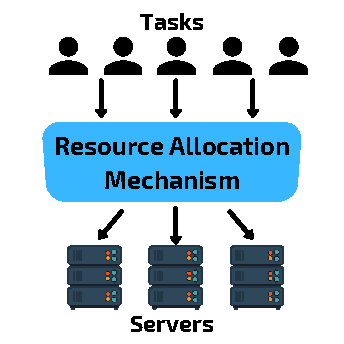
\includegraphics[width=8cm]{figures/system_model.pdf}
    \caption{System model}
    \label{fig:system_model}
\end{figure}

A sketch of the system is shown in Fig.~\ref{fig:system_model}.
We assume that in the system there is a set of $I = \{1,2,\ldots,\left|I\right|\}$ servers are heterogeneous in all
characteristics. Each server has a fixed availability of resources: storage for the code/data needed to run a task
(e.g., measured in GB), computation capacity in terms of CPU cycles per time interval (e.g., measured in FLOP/s),
and communication bandwidth to receive the data and to send back the results of the task after execution
(e.g., measured in Mbit/s). We denote these resources for server $i$: the storage capacity as $S_i$, computation
capacity as $W_i$, and the communication capacity as $R_i$.

There is a set $J = \{1,2,\ldots,\left| J \right|\}$ of  different tasks that require service from one of the servers
in set $I = \{1,2,\ldots, \left| I \right|\}$. Time is denoted by $T = \{1, 2, \ldots, \left| T \right|\}$. For a task
to be allocated to a server, $x_{i,j} = 1$ such that $x_{i,j}$ represents if a task $j$ is allocated to server $i$.
The aims of the system is to maximise task values that are completed, called the social welfare is
equation~\ref{eq:objective}. Task allocation is restricted such that only a task can only be allocated to a single task
(constraint~\ref{eq:server_task_binary} and~\ref{eq:server_task_limit}).

\begin{align}
    \text{max} \sum{j \in J} v_j \left( \sum_{i \in I} x_{i,j} \right) \label{eq:objective} \\
    x_{i,j} \in \{0, 1\} && \forall{j \in J, i \in I} \label{eq:server_task_binary} \\
    \sum_{i \in I} x_{i,j} \leq 1 && \forall{j \in J} \label{eq:server_task_limit} \\
\end{align}

%% Todo probably fixed
Due to the addition of time, modifications must be previous work in~\cite{FlexibleResourceAllocation} as tasks can
be allocated resources at each time step and tasks arrive over time.
Each task is auctioned at time step, denoted by $a_j$ and must be completed by the deadline, denoted by $d_j$.
To run any of these tasks on a server requires storing the appropriate code/data on the same server. These could be,
for example, a set of images, videos or CNN layers in identification tasks. The storage size of task $j$ is denoted
as $s_j$ with the rate at which the program is transferred at time $t$ being $s^{'}_{j,t}$. For a task to be computed
successfully, it must fetch and execute instructions on a CPU. We consider the total number of CPU cycles required
for the program to be $w_j$, where the rate at which the CPU cycles are assigned to the task at time $t$ is
$w^{'}_{j,t}$. Finally, after the task is run and the results obtained, the latter need to be sent back to the user.
The size of the results for task $j$ is denoted with $r_j$, and the rate at which they are sent back to the user
is $r^{'}_{j,t}$ at time $t$.

As each task must complete each stage is serial order (loading, computing then sending of
results) due to practical problem that server's couldn't start computing a task that was not fully loaded. This is in
comparison to previous work that allowed task stages to be completed in parallel. The progress is denoted by
$\hat{s}_{j,t}$ for the loading progress, $\hat{w}_{j,t}$ for the compute progress and $\hat{r}_{j,t}$ for the sending
progress. These variables are updated recursively from the previous value plus the resources allocated
(equations~\ref{eq:loading_progress},~\ref{eq:compute_progress} and~\ref{eq:sending_progress}). In the case of compute
progress and sending progress (equations~\ref{eq:compute_progress} and~\ref{eq:sending_progress}), resources can't be
allocated till the previous stage is completed. Therefore, the resource allocated multiple by the floor of the ratio
between the previous stage progress and the required resources of the stage. Meaning that if the previous stage is not
completed, no new resources can be allocated. For the task to be completed successfully, the sending results stage
must be completed before the task deadline (equation~\ref{eq:deadline}).

\begin{align}
    \hat{s}_{j,t+1} = \hat{s}_{j,t} + s^{'}_{j,t} &&
        \forall{j \in J, t \in \{a_j, \dots, d_j\}} \label{eq:loading_progress} \\
    \hat{w}_{j,t+1} = \hat{w}_{j,t} + w^{'}_{j,t} \left \lfloor{\frac{\hat{s}_{j,t}}{s_j}}\right \rfloor &&
        \forall{j \in J, t \in \{a_j, \dots, d_j\}} \label{eq:compute_progress} \\
    \hat{r}_{j,t+1} = \hat{r}_{j,t} + r^{'}_{j,t} \left \lfloor{\frac{\hat{s}_{j,t}}{s_j}}\right \rfloor &&
        \forall{j \in J, t \in \{a_j, \dots, d_j\}} \label{eq:sending_progress} \\

    \hat{r}_{j,d_j} = r_j && \forall{j \in J} \label{eq:deadline} \\
\end{align}

Additional constraints are to initialise the progress variables and to limit the range of valid values.
Constraints~\ref{eq:init_loading_progress},~\ref{eq:init_compute_progress} and~\ref{eq:init_sending_progress} initialise
the stage progress at the first time step of the task at $a_j$, the task auction time. To limit the range of resource
usage, two sets of constraints are used, the first is to limit the range of progress to be less than or equal to the
required resources of the task (constraints~\ref{eq:limit_loading_progress},~\ref{eq:limit_compute_progress}
and~\ref{eq:limit_sending_progress}). The second is to limit the resource usage to be a positive real number
(constraints~\ref{eq:limit_loading_usage},~\ref{eq:limit_compute_usage} and~\ref{eq:limit_sending_usage}).

\begin{align}
    \hat{s}_{j, a_j} = 0 && \forall{j \in J} \label{eq:init_loading_progress} \\
    \hat{w}_{j, a_j} = 0 && \forall{j \in J} \label{eq:init_compute_progress} \\
    \hat{r}_{j, a_j} = 0 && \forall{j \in J} \label{eq:init_sending_progress} \\

    0 \leq \hat{s}_{j,t} \leq s_j && \forall{j \in J, t \in \{a_j, \dots, d_j\}} \label{eq:limit_loading_progress} \\
    0 \leq \hat{w}_{j,t} \leq w_j && \forall{j \in J, t \in \{a_j, \dots, d_j\}} \label{eq:limit_compute_progress} \\
    0 \leq \hat{r}_{j,t} \leq r_j && \forall{j \in J, t \in \{a_j, \dots, d_j\}} \label{eq:limit_sending_progress} \\

    0 \leq s^{j,t} < \infty && \forall{j in J, t \in T} \label{eq:limit_loading_usage} \\
    0 \leq w^{j,t} < \infty && \forall{j in J, t \in T} \label{eq:limit_compute_usage} \\
    0 \leq r^{j,t} < \infty && \forall{j in J, t \in T} \label{eq:limit_sending_usage} \\
\end{align}

As server have limited capacity, the total resource usages for all tasks running on a server must be capped.
The storage constraint (equation~\eqref{eq:server_storage_capacity}) is unique as the previous amount
loaded in kept till the end of a program on server. While the computation capacity
(equation~\eqref{eq:server_computation_capacity} is the sum of compute used by all of the tasks on a server $i$ at
time $t$ and the bandwidth capacity (equation~\eqref{eq:server_bandwidth_capacity}) is the sum of loading and sending
usages by tasks.

\begin{align}
    \sum_{j \in J} \hat{s}_{j,t} \dot x_{i,j} \leq S_i, &&
        \forall{i \in I, t \in T} \label{eq:server_storage_capacity} \\
    \sum_{j \in J} w^{'}_{j,t} \dot x_{i,j} \leq W_i, &&
        \forall{i \in I, t \in T} \label{eq:server_computation_capacity} \\
    \sum_{j \in J} (s^{'}_{j,t} + r^{'}_{j,t}) \dot x_{i,j} \leq R_i, &&
        \forall{i \in I, t \in T} \label{eq:server_bandwidth_capacity} \\
\end{align}

\section{Auctioning of Tasks}\label{sec:auctioning-of-tasks}
While the mathematical description of the problem presented above doesn't contain any auctioning properties as it
aims to maximise the social welfare, in real life cloud providers normally wish to be paid to the use of their services.
However all of auction mechanisms that were discussed in section~\ref{sec:related-work-in-cloud-computing} are not
applicable as the metrics used to calculate the cost, total resource usage or server resource demand are not possible
to compute prior to the task starting. Because of this, a novel or modified auction mechanism must be used to deal with
these changes. Due to the complexities of devising new auction mechanism and the large corpus of research on auctions,
this project has chosen to use the Vickrey auction~\citep{vickrey}. This decision is justified in
section~\ref{sec:justification-of-vickrey-auction-mechanisms} on why this auction was chosen over other alternatives.

The modifications made to the Vickrey auction is to reverse the auction as server are bidding on tasks instead of
a task buying servers. Meaning that the server with the minimum price is wins the task with the task paying the
second minimum price. Because of this, the auction is referenced to as the reverse Vickrey auction. The auction works
by allowing servers to all submit their bid for the task with the winner being the server with the lowest
price but actually gains the second lowest price which the task pays. The advantage of using the Vickrey auction is
that it is incentive compatible meaning that the dominant strategy for bidding on a task is to bid your truthful value.
This should help server as they dont need to learn how to outbid another agent as it only needs to consider its own
evaluation. This also allows agents to learn through self-play effectively. A second advantage is that the auction only
a single round of bidding compared to alternative auctions like English or Dutch auctions. This makes auctioning fast
no matter the number of servers. An advantage for tasks is reverse price can be put in place to prevent servers from
bidding to high however this is believed to be unnecessary as it wouldn't affect how server's bid.

\section{Proposed Agents}\label{sec:proposed-agents}
Using the optimisation formulation and vickrey auction explained in the previous two sections, a solution for the
project can be devised. To model the solution, a markov decision process (MDP)~\cite{Bel} is used as this is a common
method of describing discrete time stochastic processes from the perspective of an individual agent.
Figure~\ref{fig:mdp_system_model} is a MDP model for this project with the auction and resource allocation sections
separated out. This is important as server can't have a single agent for both sections as the policies have both
different state space and reward functions. Because of this, each agent is imagined to exist in solely the auction
environment or the resource allocation environment as the agents can't be trained on the whole environment.
Therefore unique agents are proposed for each environment, auction agents in
subsection~\ref{subsec:proposed-auction-agents} and resource allocation agents
in~\ref{subsec:proposed-resource-allocation-agents}.

\begin{figure}
    \centering
    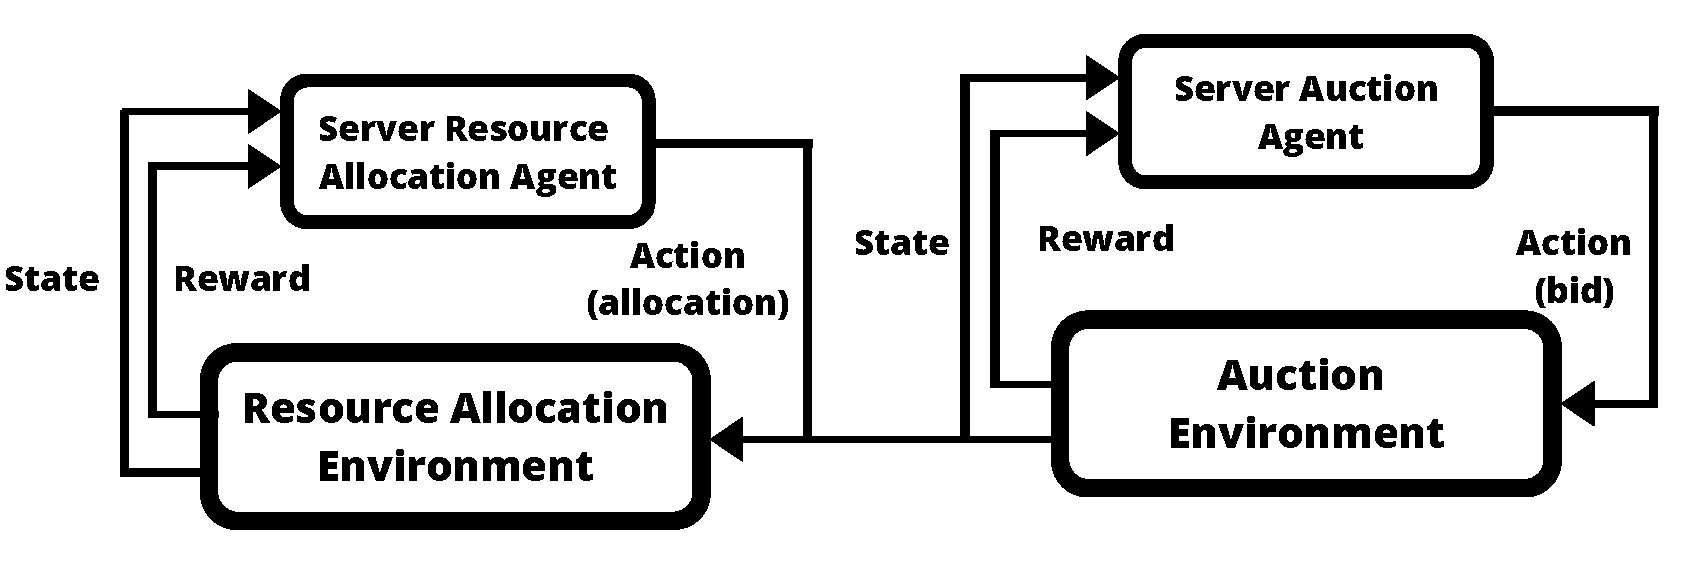
\includegraphics[width=14cm]{figures/flexible_resource_allocation_env.pdf}
    \caption{Markov Decision process system model}
    \label{fig:mdp_system_model}
\end{figure}

This author believes this environment is particularly interesting in multi-agent reinforcement learning due to the fact
that the aim of the environment is cooperative (to maximise the social welfare) but the servers (auction agents) are in
competition to maximise their individual profits. But then the resource allocation agent must be cooperative in its
actions to allocate resources to each task as the server wish to complete as many tasks as they can.

\subsection{Proposed auction agents}\label{subsec:proposed-auction-agents}
Traditionally pricing mechanisms~\citep{al2013cloud} rely on mixture of metrics: resource availability, resource demand,
quality of service, task resource requirements, task resource allocation quantity, etc. However these metrics are
difficult to approximate at the point of server bidding due to the unknown task resource usage of any task in the
future without restricting possible rebalancing of tasks in the future. Therefore to derive a price function would wish
to take into account a range of attributes like server capacity, progress of currently allocated tasks, availability
of future tasks and the required of the task being auctioned. Therefore due to the expected complexity of this function,
reinforcement learning, a subset of machine learning, is proposed as a method to learn neural networks that are
universal function appromixated approximators~\citep{csaji2001approximation}. Meaning that these agents can learn
without human support the optimal pricing function to maximise server profits. In conjunction to this, simple
heuristics will also be implemented in order compare the effectiveness of the reinforcement learning to untrained
heuristics.

Due to the auction environment having a discrete state space and a continuous action space, both policy gradient and
deep q networks are feasible training methods. A explanation of these algorithm are described in
section~\ref{sec:related-work-in-machine-learning}. Therefore a deep deterministic policy gradient~\citep{ddpg}
agent and deep q networks~\cite{atari} (with a discretized action space) will be implemented in order to compare the
agent capability. While the state space is discrete, it is not fixed, actions dont have a fixed number of tasks
already allocated to a server therefore the neural networks proposed for these agents require recurrent neural networks.
Because of this, a long/short term memory (LSTM) layer will be first layer of the network, piping to linearly
activated neurons for the deep q and critic networks and ReLU activated neurons for the policy gradient actor networks.

\subsection{Proposed resource allocation agents}\label{subsec:proposed-resource-allocation-agents}
At each time step, the server has the ability to redistribute it resources between its allocated tasks. While this
problem isn't believed to be as complex as the pricing function due to being a cooperative function rather than a
competitive function. However due to the complexity of knowing how to allocate resources between multiple tasks at the
same time, both deep q networks and policy gradient agents will be implemented.

However a similar problem exists to the proposed auction agents (in subsection~\ref{subsec:proposed-auction-agents}) as
to know how to allocate resources to be single task is be aware of the other tasks that the server currently contains.
Therefore a similar network is proposed to allow for the other tasks to be passed in in order to compare the current
task having resources allocated to and the other tasks also allocated to the server. The only other change is that
the action space doesn't represent the equivalent amount of a certain type of resources but instead the weighting
for that resources. This is as if the network wanted to allocate as many resources as possible while having to keep
the total amount of resource under the total available then this is extremely difficult. Therefore the action space
instead represents the weight of that resource with the equivalent amount of resources can then be determined by the
server. This aims to reduce the needed complexity of the resource allocation function and speed up the learning time
of the agent.
